\documentclass{article}%
\usepackage[T1]{fontenc}%
\usepackage[utf8]{inputenc}%
\usepackage{lmodern}%
\usepackage{textcomp}%
\usepackage{lastpage}%
\usepackage{graphicx}%
%
\title{IntroductiontoDatabases}%
\author{Notepal}%
\date{\today}%
%
\begin{document}%
\normalsize%
\maketitle%
\section{Note1}%
\label{sec:Note1}%
\subsection{Page 1}%
\label{subsec:Page 1}%


\begin{figure}[h!]%
\centering%
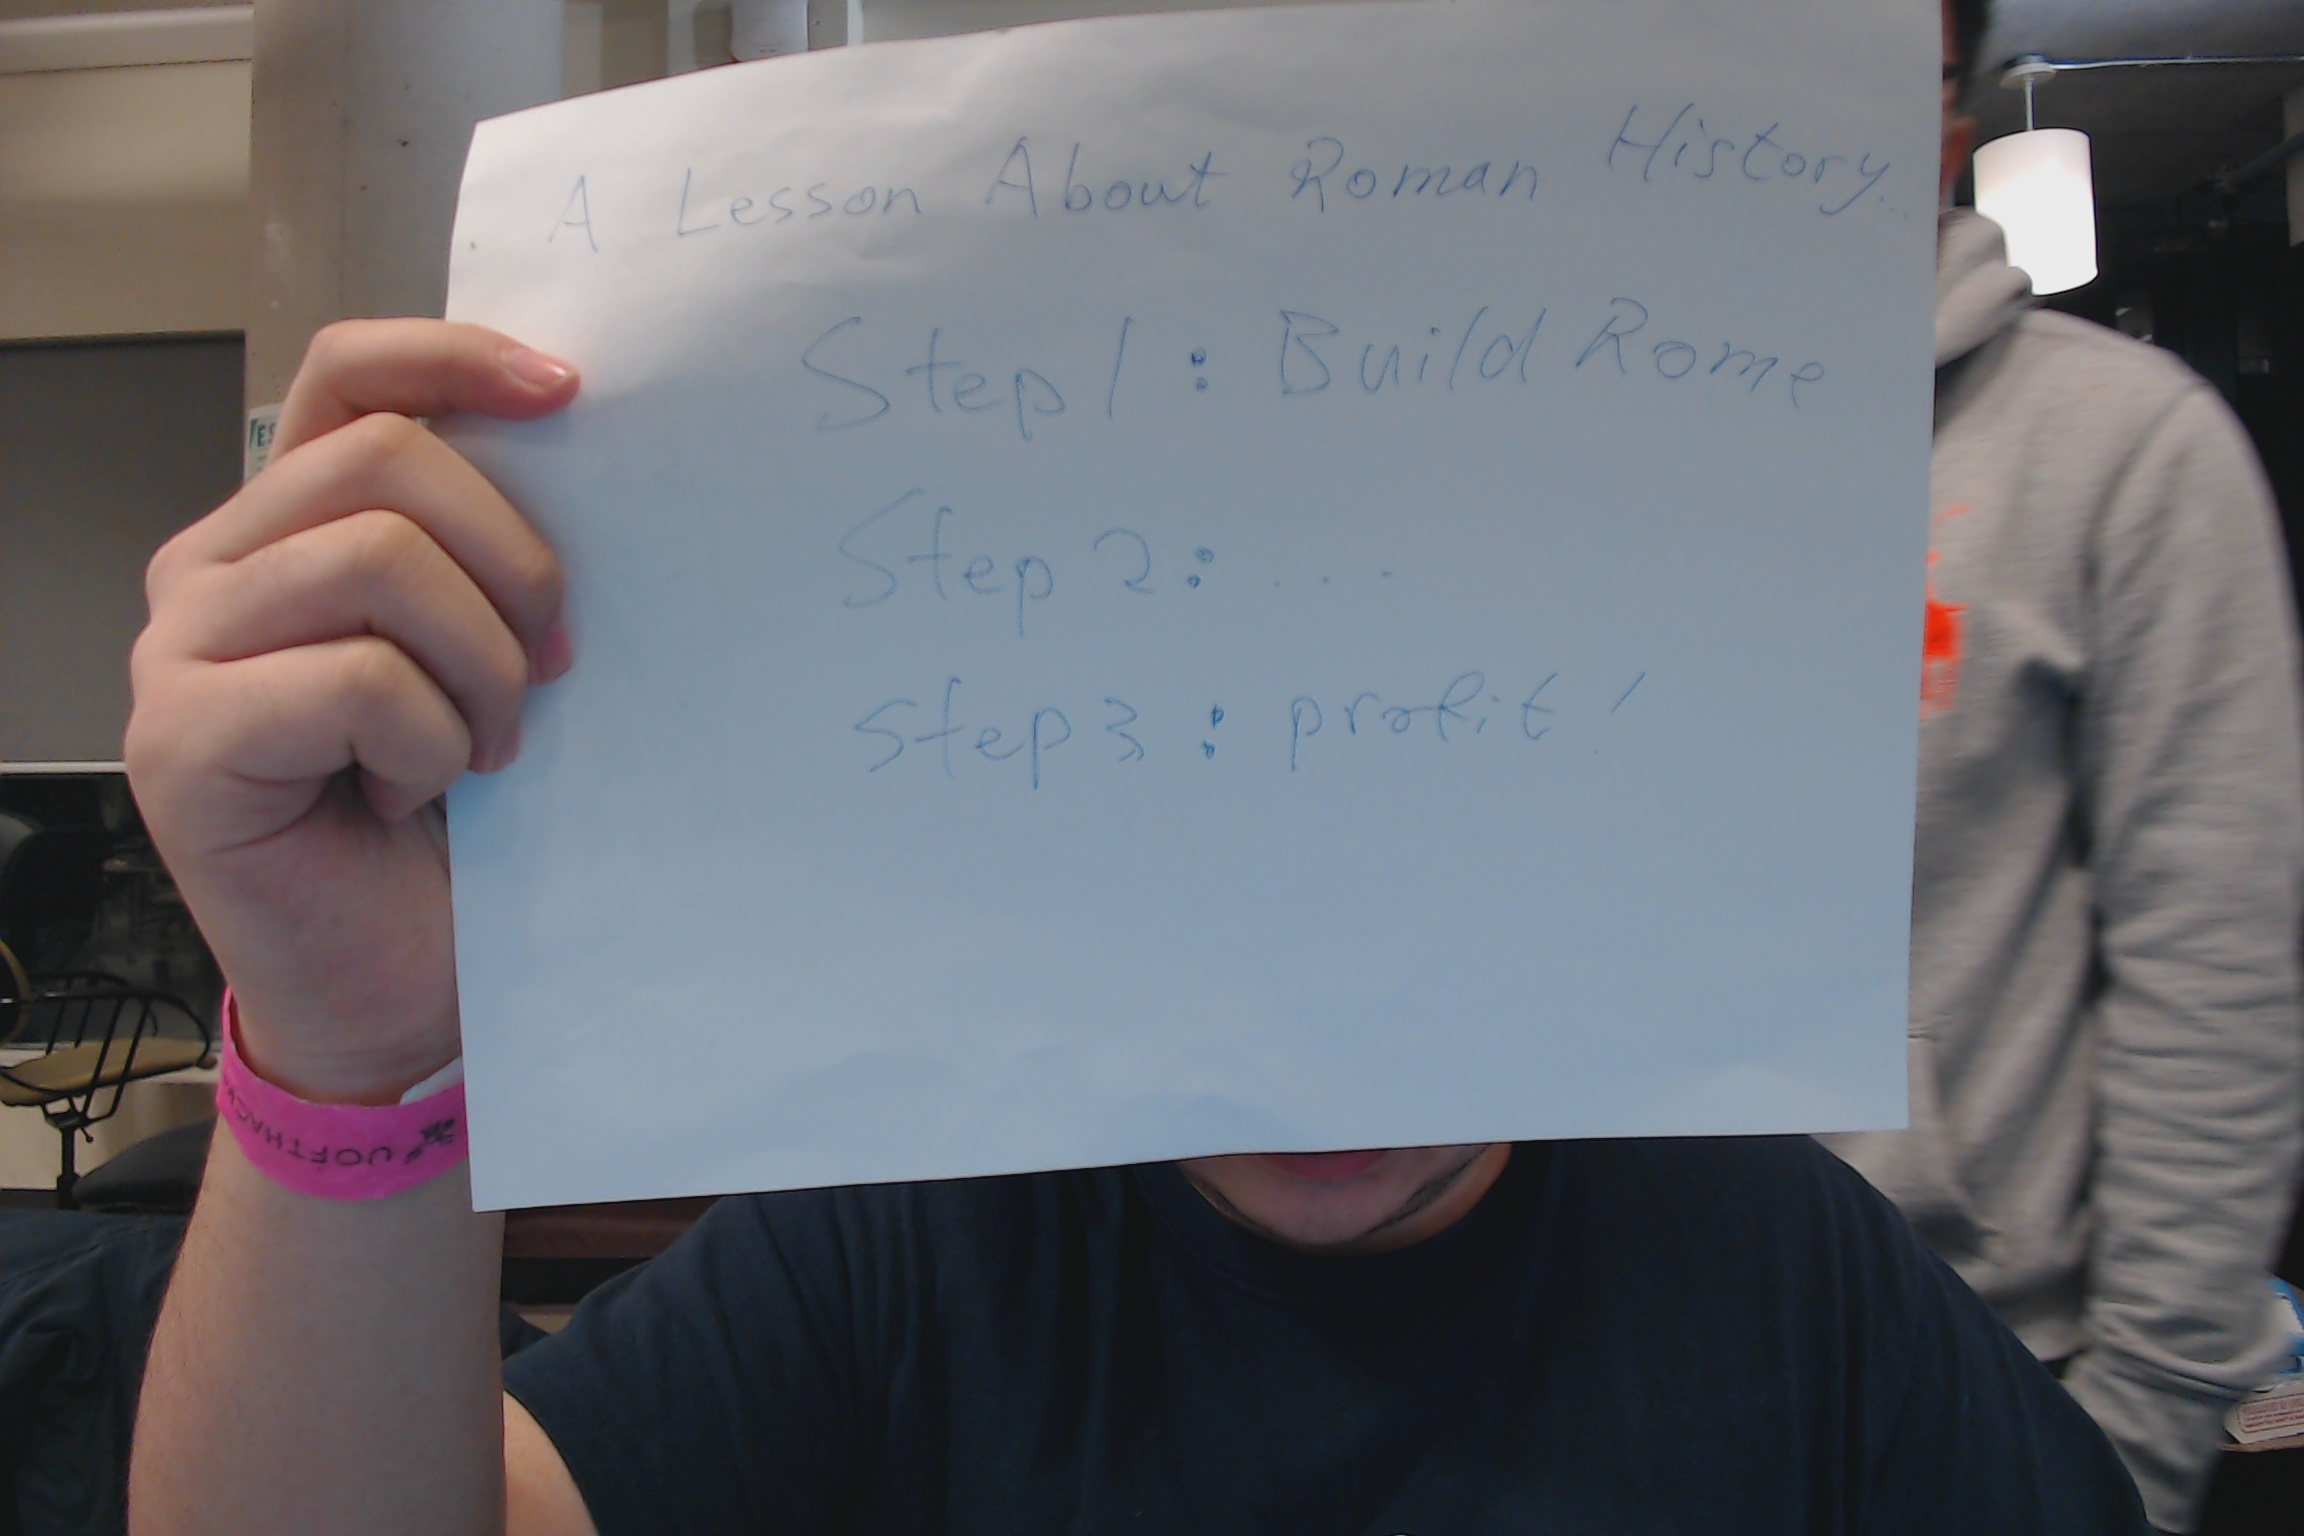
\includegraphics[width=300px]{../Notes/IntroductiontoDatabases/Note1/image1.jpg}%
\caption{Image 1}%
\end{figure}

%
Okay, so good morning everyone today. We're going to talk a little bit about the use of SQL in relational databases and what it is and why it's important to development. \newline%
 next page \newline%

%
\section{Note1}%
\label{sec:Note1}%
\subsection{Page 2}%
\label{subsec:Page 2}%


\begin{figure}[h!]%
\centering%
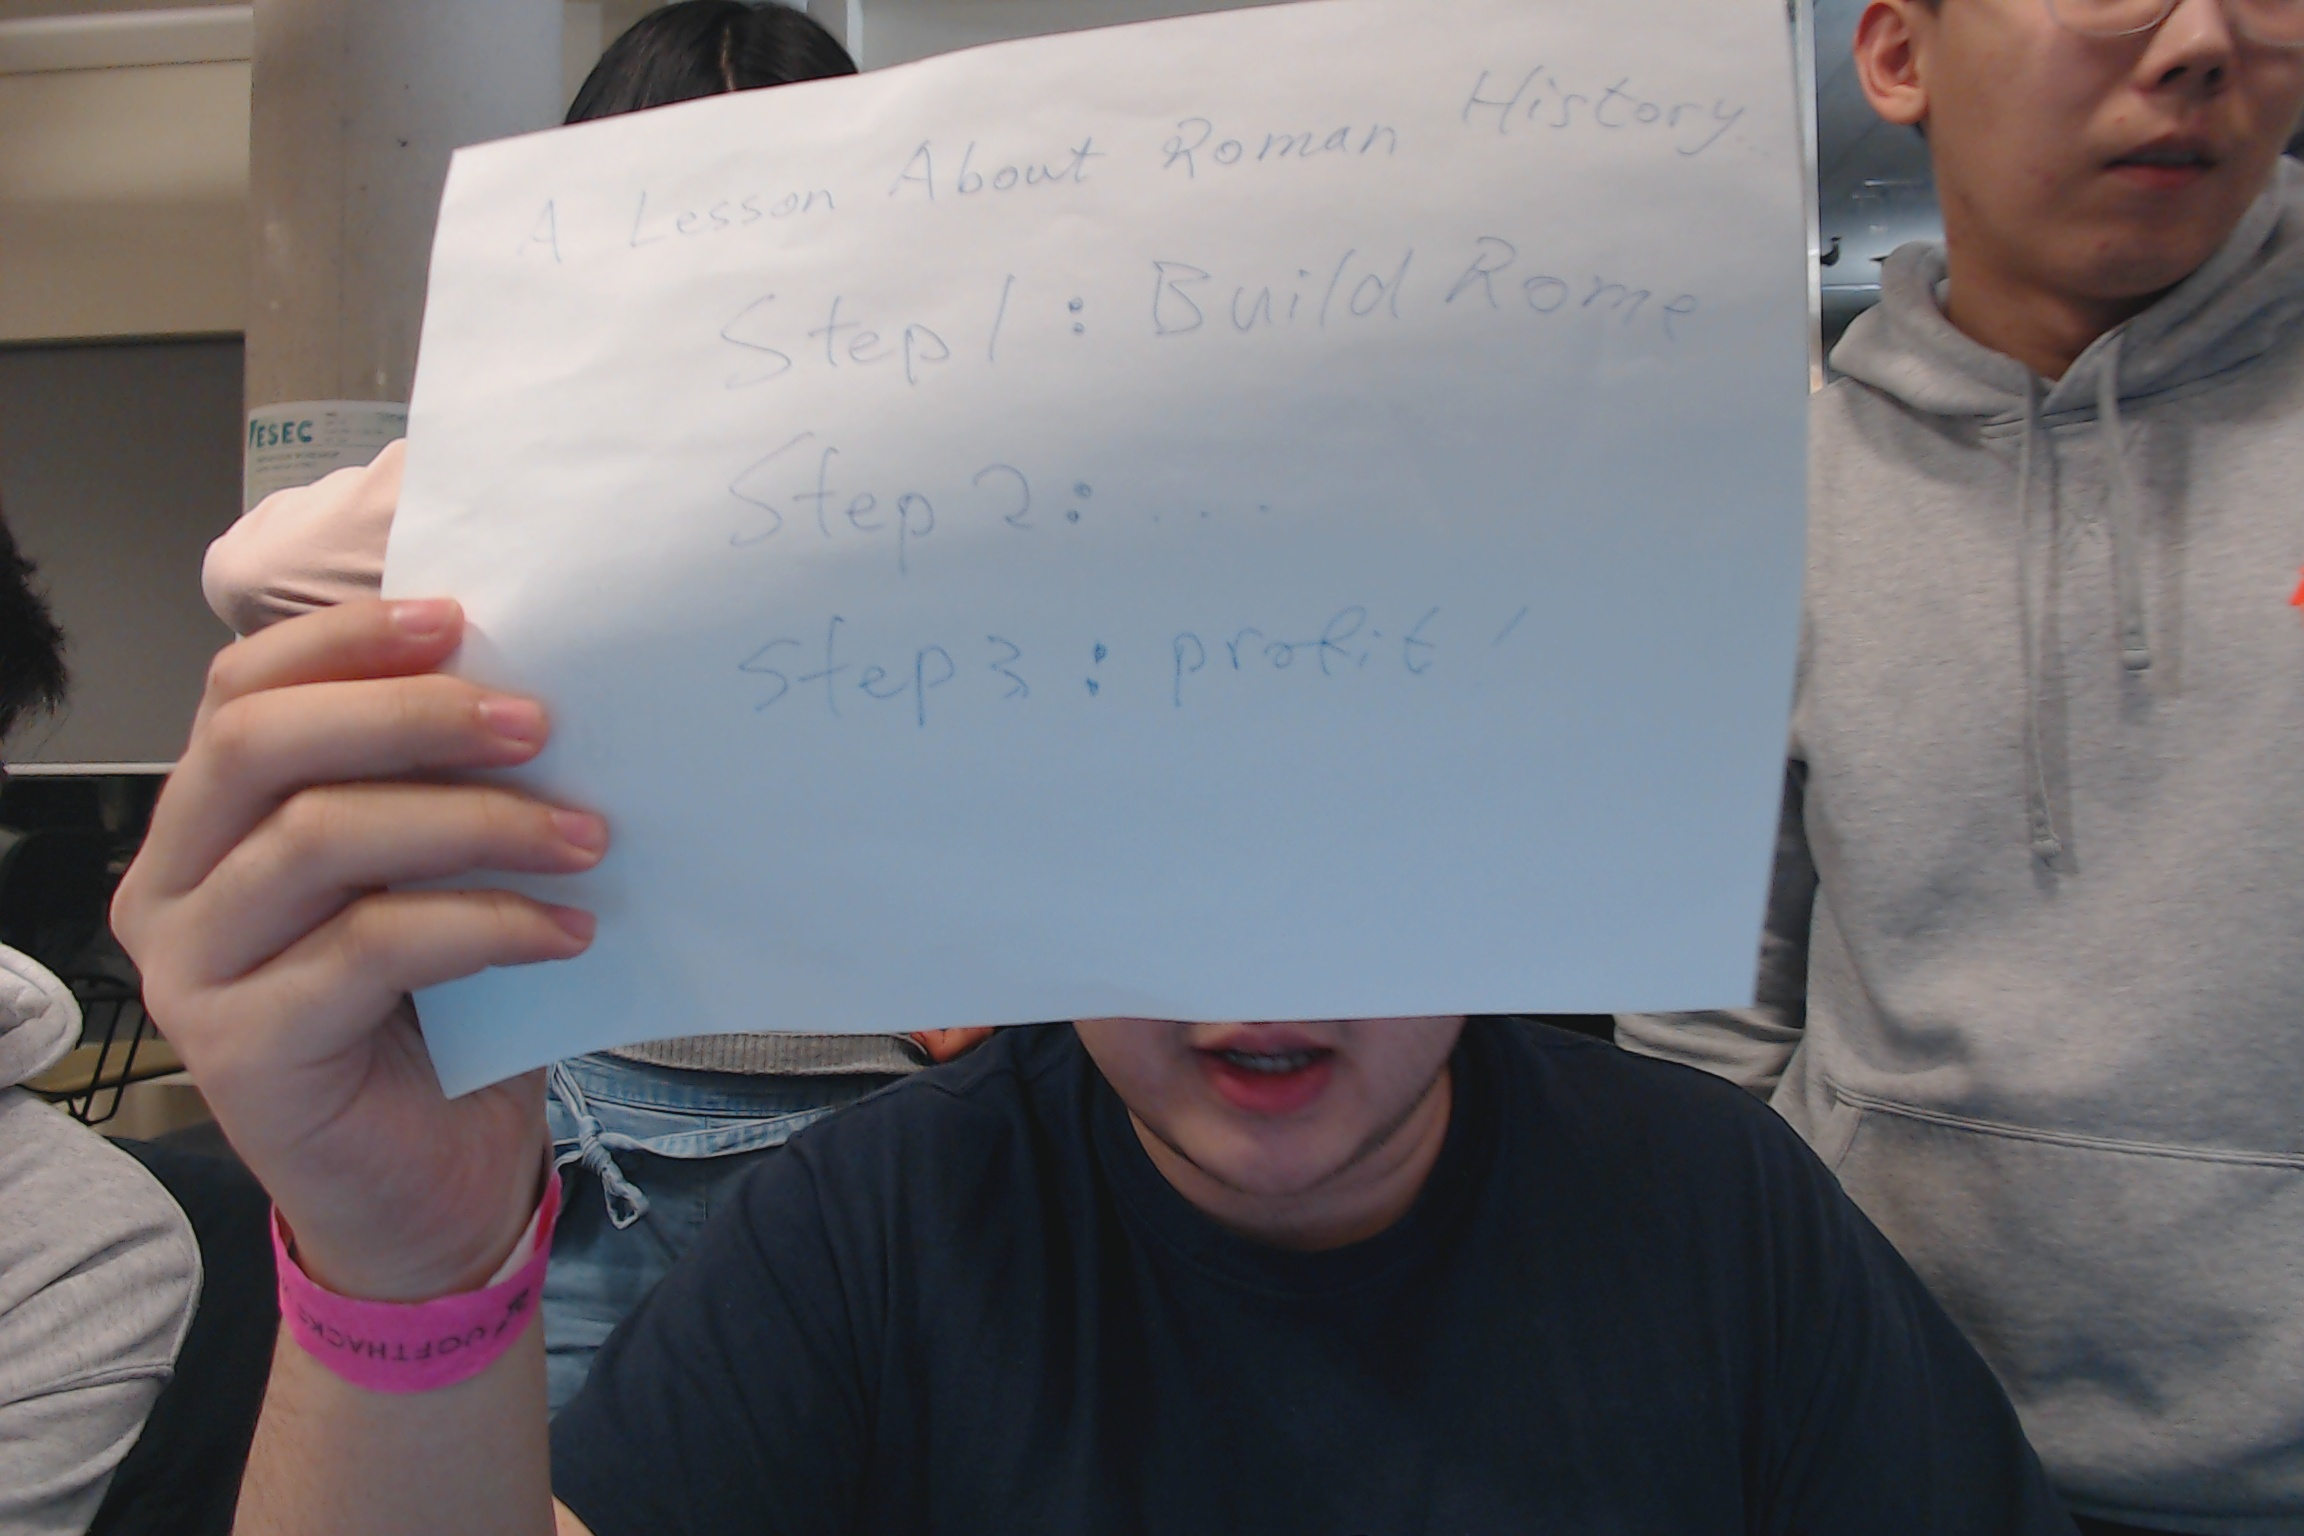
\includegraphics[width=300px]{../Notes/IntroductiontoDatabases/Note1/image2.jpg}%
\caption{Image 2}%
\end{figure}

%
So to continue our conversation from the last board, we need to really talk a little bit more about relational. What are tusken Raiders? \newline%

%
\section{Note1}%
\label{sec:Note1}%
\subsection{Page 3}%
\label{subsec:Page 3}%


\begin{figure}[h!]%
\centering%
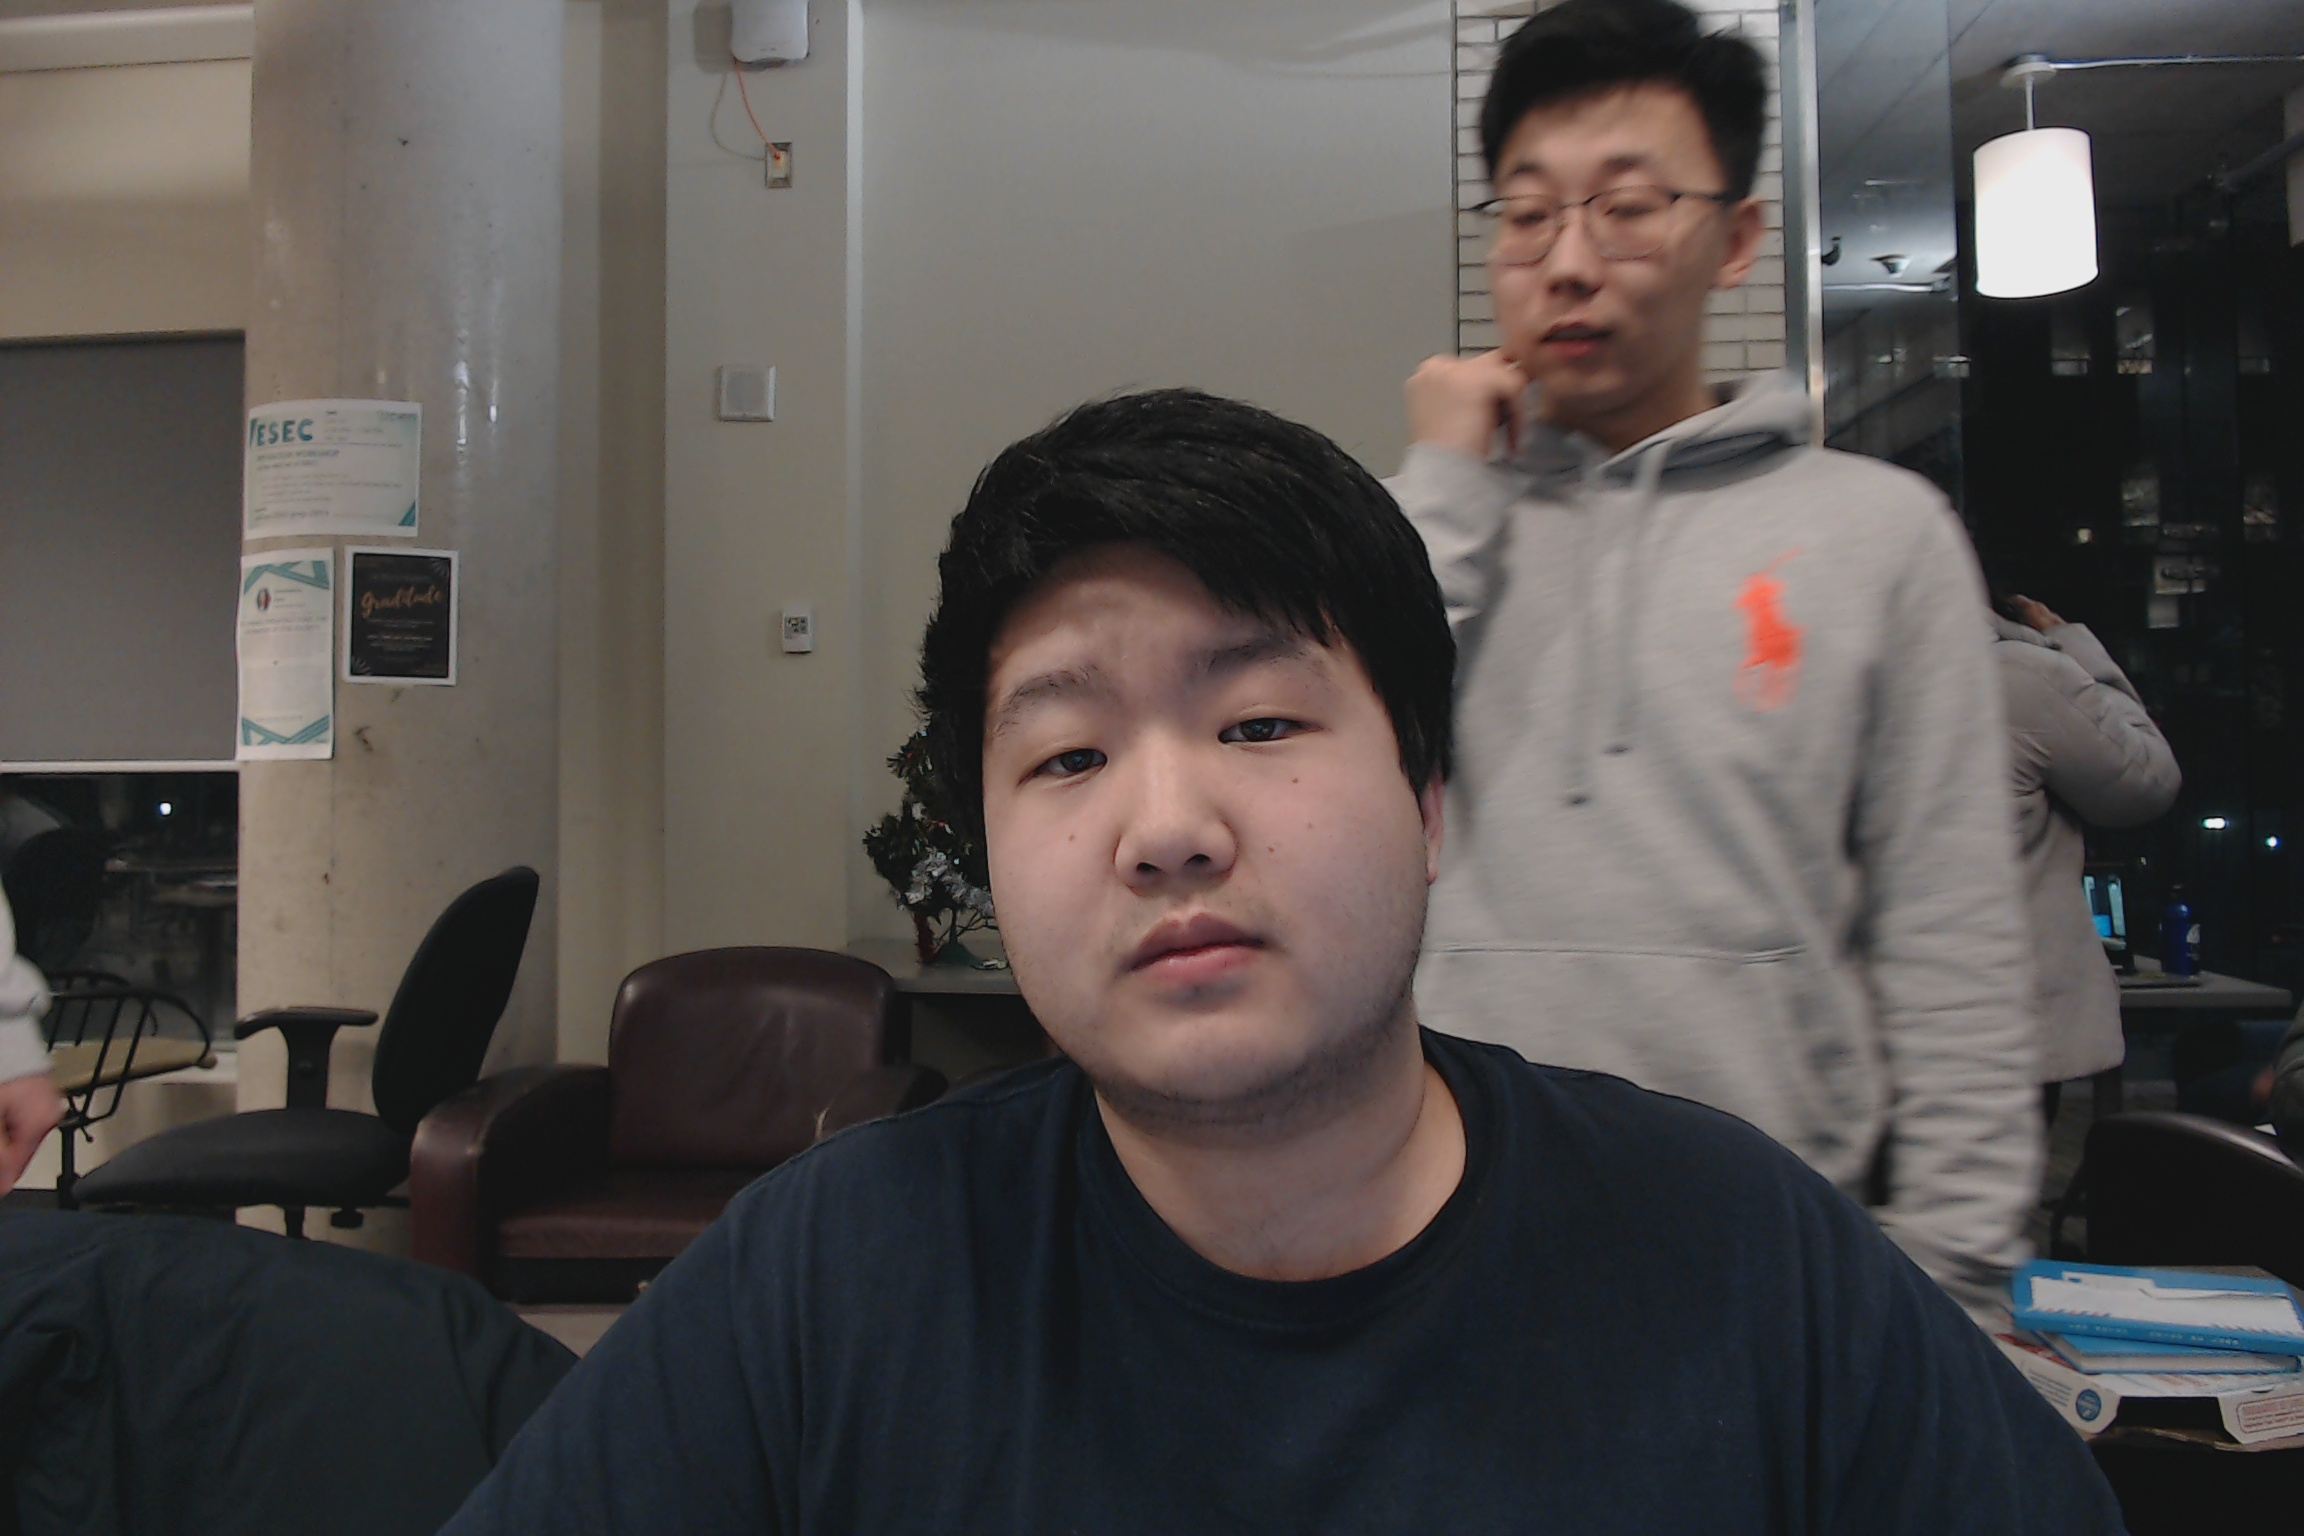
\includegraphics[width=300px]{../Notes/IntroductiontoDatabases/Note1/image3.jpg}%
\caption{Image 3}%
\end{figure}

%
By accident, but now I'm going to end. \newline%
 and the note \newline%

%
\end{document}